% Compile with Tectonic:
%   conda run -n alphagenome tectonic docs/rna_seq11_collaborator_update_20260604_zh_compact.tex
\documentclass[UTF8,aspectratio=169,10pt]{ctexbeamer}

\usetheme{Boadilla}
\usecolortheme{dolphin}
\setbeamertemplate{navigation symbols}{}
\setbeamertemplate{footline}[frame number]

\usepackage{booktabs}
\usepackage{array}
\usepackage{tikz}
\usetikzlibrary{arrows.meta,positioning}

\definecolor{agblue}{RGB}{38,88,156}
\definecolor{aggreen}{RGB}{37,125,97}
\definecolor{agred}{RGB}{174,74,65}
\definecolor{aggray}{RGB}{92,102,112}

\setbeamercolor{title}{fg=agblue}
\setbeamercolor{frametitle}{fg=agblue}
\setbeamercolor{structure}{fg=agblue}
\setbeamercolor{block title}{fg=white,bg=agblue!82}
\setbeamercolor{block body}{bg=agblue!5}

\newcommand{\smallnote}[1]{\vspace{0.35em}{\scriptsize\color{aggray}#1}}

\title[C. elegans RNA-seq11 Adapter Update]{C. elegans RNA-seq11 Adapter 最新进展}
\subtitle{从可工作的 128bp 基线到面向生物信号的 1bp residual 模型}
\author{Ziyang Huang}
\date{2026-06-04}

\begin{document}

\begin{frame}
  \titlepage
\end{frame}

\begin{frame}{上次的结论是：128bp adapter 已经可用，但还只是起点}
  \begin{itemize}
    \item Frozen AlphaGenome trunk + 128bp RNA-seq adapter 已经能工作。
    \item 数据是 11 个 grouped C. elegans RNA-seq tracks。
    \item 染色体划分保持不变：train 为 I--IV，valid 为 V，test 为 X。
    \item 上次选中的模型：valid MSE 1.06099，Pearson 0.58810。
    \item 当时 1bp adapter 和 LoRA pilots 都还没有超过 128bp adapter。
  \end{itemize}

  \smallnote{本次汇报承接上次 128bp baseline；后续模型选择仍只基于 validation split。}
\end{frame}

\begin{frame}{旧 128bp 基线并没有饱和}
  \centering
  \begin{tabular}{p{0.28\textwidth}ccp{0.34\textwidth}}
    \toprule
    模型 & Valid MSE & Pearson & 主要变化 \\
    \midrule
    Old 128bp baseline & 1.06099 & 0.58810 & 第一个可工作的 adapter \\
    Improved 128bp model & 0.88033 & 0.67392 & 更好的 head、loss 和 schedule \\
    \bottomrule
  \end{tabular}

  \vspace{1.1em}
  \begin{block}{结论}
    在改变 representation strategy 之前，只通过更合适的 objective 和 schedule，valid MSE 已经从 1.06099 明显降到 0.88033。
  \end{block}
\end{frame}

\begin{frame}{1bp 信息在 residual correction 里变得有用}
  \centering
  \begin{tabular}{p{0.36\textwidth}cc}
    \toprule
    模型 & Valid MSE & Pearson \\
    \midrule
    Improved 128bp model & 0.88033 & 0.67392 \\
    1bp residual model & \textbf{0.83558} & \textbf{0.69463} \\
    \bottomrule
  \end{tabular}

  \vspace{1.1em}
  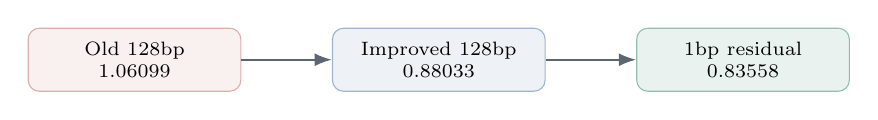
\begin{tikzpicture}[
    font=\scriptsize,
    node distance=1.15cm,
    msebox/.style={draw,rounded corners,align=center,minimum width=2.7cm,minimum height=0.8cm},
    arrow/.style={-{Latex[length=2.2mm]},thick,aggray}
  ]
    \node[msebox,fill=agred!8,draw=agred!45] (old) {Old 128bp\\1.06099};
    \node[msebox,fill=agblue!8,draw=agblue!45,right=of old] (imp) {Improved 128bp\\0.88033};
    \node[msebox,fill=aggreen!10,draw=aggreen!50,right=of imp] (res) {1bp residual\\0.83558};
    \draw[arrow] (old) -- (imp);
    \draw[arrow] (imp) -- (res);
  \end{tikzpicture}

  \begin{itemize}
    \item 早期 naive 1bp pilots 没有赢。
    \item 但在强 128bp base 上叠加 1bp residual correction，validation performance 明确提升。
    \item 因此 1bp 更适合作为 correction layer，而不是直接替代 128bp。
  \end{itemize}
\end{frame}

\begin{frame}{最好的模型已经进入一个很窄的 plateau}
  \begin{block}{Top15 的共同模式}
    \begin{itemize}
      \item Top15 模型全部是同一策略的变体：frozen 128bp prediction + 1bp residual correction。
      \item Top15 full-MSE spread 只有约 0.00137。
      \item 模型差异主要来自 warm-start、learning rate、beta 和 track weights。
    \end{itemize}
  \end{block}

  \begin{block}{解释}
    继续做同方向的小型 continuation run 不太可能解决剩下的生物学错误；问题已经从“能不能预测 RNA-seq”转向“哪些重要信号还没学好”。
  \end{block}
\end{frame}

\begin{frame}{当前最佳模型仍然漏掉关键生物信号}
  \centering
  \begin{tabular}{lc}
    \toprule
    失败模式 & Metric \\
    \midrule
    High $>3$ signal MSE & 4.9257 \\
    Top 5\% true signal MSE & 5.8610 \\
    Top 1\% true signal MSE & 10.8414 \\
    Exon MSE & 1.6658 \\
    Gene-body MSE & 1.1104 \\
    Gene-level Spearman & 0.5835 \\
    Local-gradient Pearson & 0.3451 \\
    \bottomrule
  \end{tabular}

  \vspace{0.8em}
  \begin{block}{结论}
    Global MSE 已经改善，但 high-expression amplitude、exon/gene-body regions、intestine tracks 和 local boundaries 仍然偏弱。
  \end{block}
\end{frame}

\begin{frame}{Signal-weighted loss 能改善 amplitude，但有代价}
  \centering
  \begin{tabular}{p{0.31\textwidth}cccc}
    \toprule
    模型 & Full MSE & high\_gt3 MSE & top5 MSE & top1 MSE \\
    \midrule
    1bp residual reference & \textbf{0.8356} & 4.9257 & 5.8610 & 10.8414 \\
    Signal top5x3 & 0.8632 & \textbf{4.1605} & \textbf{4.9061} & \textbf{9.2685} \\
    Signal intestine-high & 0.8531 & 4.3510 & 5.1905 & 9.8277 \\
    \bottomrule
  \end{tabular}

  \vspace{0.8em}
  \begin{block}{结论}
    Signal weighting 可以恢复 high-expression amplitude，但会牺牲 global MSE。它应被视为 high-signal / intestine co-winner，而不是 all-purpose model。
  \end{block}
\end{frame}

\begin{frame}{Region-weighted loss 能改善 exon 和 gene-body 信号}
  \centering
  \begin{tabular}{p{0.30\textwidth}cccc}
    \toprule
    模型 & Full MSE & Exon MSE & Gene-body MSE & Intergenic MSE \\
    \midrule
    Reference & \textbf{0.8356} & 1.6658 & 1.1104 & \textbf{0.2980} \\
    Region exon-gene v2 & 0.8367 & 1.6591 & 1.1083 & 0.3048 \\
    Region exon-gene v1 & 0.8377 & \textbf{1.6550} & \textbf{1.1079} & 0.3084 \\
    \bottomrule
  \end{tabular}

  \vspace{0.8em}
  \begin{block}{结论}
    Region weighting 直接降低 exon/gene-body error。v2 是更平衡的 biological-utility candidate；v1 是最强的 exon/gene-body candidate。
  \end{block}
\end{frame}

\begin{frame}{Gene auxiliary loss 和 calibration 还不是主方向}
  \begin{itemize}
    \item Gene auxiliary loss $\lambda=0.03$ 在测试设置下没有改善 gene-body mean MSE。
    \item 因为低 lambda 没有出现正向 gene-MSE signal，更大的 lambda 值没有被优先推进。
    \item Track-affine output calibration 只带来小幅 amplitude 改善，没有形成明确的新 winner。
  \end{itemize}

  \vspace{0.8em}
  \begin{block}{结论}
    Gene auxiliary loss 和 calibration 是有用的工具，但不是当前最主要的推进方向。
  \end{block}
\end{frame}

\begin{frame}{171 个 checkpoint 被重新做了 validation-only 诊断}
  \begin{block}{重新评估的内容}
    \begin{itemize}
      \item full MSE / Pearson，作为 sanity reference
      \item gene-level Pearson / Spearman
      \item high-signal top1 / top5 amplitude
      \item exon / gene-body / intergenic regions
      \item intestine T1/T3/T4
      \item 128bp 和 1kb pooled metrics
      \item downstream gene-profile probe
    \end{itemize}
  \end{block}

  \begin{block}{目的}
    所有评估都保持 validation-only；目标是判断哪个模型更能保留有用的 biological signal，而不只是哪个模型 pixel-level MSE 最低。
  \end{block}

  \smallnote{完整 run path 已记录在 docs；正文不堆长 run directory。}
\end{frame}

\begin{frame}{最终解释应该是一组 purpose-specific winners}
  \centering
  \small
  \begin{tabular}{p{0.24\textwidth}p{0.26\textwidth}p{0.40\textwidth}}
    \toprule
    角色 & 模型 & 原因 \\
    \midrule
    MSE 参考 & 1bp residual rank1 & full MSE 最低，0.83558 \\
    主要生物 utility 候选 & Region exon-gene v2 & utility 最平衡，MSE 代价很小 \\
    exon/gene-body winner & Region exon-gene v1 & exon/gene-body metrics 最好 \\
    high-signal winner & Signal top5x3 & high-expression amplitude 最强 \\
    intestine high-signal winner & Intestine-high weighted & intestine high-signal behavior 最好 \\
    \bottomrule
  \end{tabular}

  \vspace{0.8em}
  \begin{block}{结论}
    MSE winner 仍然重要，但它不是唯一具有 biological utility 的模型。
  \end{block}
\end{frame}

\begin{frame}{Take-home message：下一步应按用途选模型}
  \begin{itemize}
    \item 我们从上次 128bp baseline 的 MSE 1.06099，提高到更强 128bp 训练和 1bp residual correction 的 0.83558。
    \item Diagnostics 显示剩余瓶颈是 biologically important signal：high expression、exon/gene-body regions 和 intestine tracks。
    \item Region-weighted 与 signal-weighted objectives 找到了可用于 downstream biological interpretation 的 co-winners。
  \end{itemize}

  \vspace{0.9em}
  \begin{block}{下一步}
    保留 1bp residual MSE winner 作为 reference；使用 region-weighted model 作为 main biological-utility candidate；在 high-expression / intestine-focused analyses 中使用 signal-weighted models。
  \end{block}
\end{frame}

\end{document}
